\chapter{Introduction} \label{chap:intro}

Although the basic chemical mechanisms of cellular biology are now well-known, we are still a long way from understanding how most observable characteristics of a cell or organism -- called \textit{phenotypes} -- emerge from these basic mechanisms. Advances within the last decades are now enabling high-dimensional measurements of cells, thereby allowing us to study this emergent complexity.  For example, within the last decade, RNA-sequencing (RNA-seq) has become a ubiquitous technology for measuring the set of all RNA gene products in a cell or biological sample -- called the \textit{transcriptome} -- thereby providing a snapshot of the gene activity across the entire genome (\citealp{Wang2009}).  An improvement in our ability to predict how phenotypes emerge from the complex patterns of gene activation, as captured by RNA-seq, would lead to considerable medical and technological advancements in such areas as stem cell therapy development (\citealp{Cahan, Morris2014}), disease diagnosis (\citealp{Kegerreis2019, Bryon2016, Saddiki2015, Marisa2013, Chuang2007}), and biological data analysis (\citealp{Hou2019, Alavi2018, Ellis}).  This task, which we refer to as \textit{transcriptome-based cellular phenotyping} (TBCP), is the focus of this dissertation.

Currently, it remains intractable to perform TBCP manually due to both the high number of genes (tens of thousands in the human genome) and our incomplete understanding of how the myriads of interactions between genes, proteins, and other molecules in the cell form complex systems and feedback loops.  Thus, computational approaches are required. Furthermore, biological systems are inherently noisy, so these computational approaches must take this noise into account if they are to be successful. In this dissertation, we explore the use of \textit{machine learning} --  the study of algorithms that learn by example -- for building automated TBCP systems.  Machine learning is an apt approach for overcoming the noise inherent in RNA-seq data because incorporating uncertainty is fundamental to machine learning algorithms (\citealp{Ghahramani2015}).  Furthermore, since machine learning algorithms learn from examples, these approaches provide a path to overcoming the lack of knowledge regarding the specific rules and patterns that lead from gene activity to phenotype. 
 
Although machine learning algorithms do not require a priori knowledge, they do require training examples.  In the case of applying machine learning to TBCP with RNA-seq, this entails providing the algorithm with RNA-seq data from many biological samples where each sample is labelled with a phenotype.  Unfortunately, it remains difficult for a single laboratory to produce sufficient data to train such algorithms because sample collection, preparation, and RNA-sequencing are expensive and involved processes. Fortunately, the National Institutes of Health (NIH) have created public databases where scientists who perform RNA-seq deposit their data so that other scientists can perform secondary analyses. These databases thus provide a valuable source of training data for the TBCP task.

Unfortunately, it has hitherto been challenging to utilize these public data sources due to their poorly structured metadata and heterogeneity.  In this dissertation we present three projects that address these challenges and span multiple stages of the machine learning pipeline, from the acquisition of training data to model development. These projects support the following thesis:
\begin{quote}
Large-scale, heterogeneous repositories of RNA-seq data can be leveraged to train machine learning classifiers to perform transcriptome-based cellular phenotyping.
\end{quote}
Most of this work targets the Sequence Read Archive (SRA), the premier repository of public RNA-seq data, which is curated by the NIH (\citealp{Leinonen2011}); however, this work may also be applied to other large, related databases including the Gene Expression Omnibus (\citealp{Barrett2013}).  Together, these projects advance the state-of-the-art in both our ability to leverage public data and to perform TBCP. 

In the following sections, we provide relevant background on RNA-seq, applications of TBCP, and relevant computational approaches.  The purpose of this introduction is to bridge the gap between computer scientists, biologists, and bioinformaticians.



\section{Transcriptomic analysis with RNA-seq}

Each cell in an organism contains a copy of its genome: a long sequence of four molecules, adenine (A), thymine (T), guanine (G), and cytosine (C), called DNA.  Specific subsequences along the genome are called \textit{genes} and store the instructions for constructing functional molecules, predominantly \textit{proteins}, that orchestrate the cell's chemistry\footnote{The human genome encodes approximately 20,000 protein-coding genes.}. When a gene is \textit{expressed} by the cell (i.e. used to create a protein), the gene's sequence is first copied to an intermediate information-storing molecule, called RNA, in a process called \textit{transcription} . These RNA molecules, called \textit{transcripts}, are free to float away from the DNA where they bind with cellular machinery, called \textit{ribosomes}, which are responsible for converting the transcript's sequence into a protein\footnote{Some genes do not encode for a protein. Rather, the RNA itself performs a function in the cell. These RNA are often called \textit{non-coding RNA's}.}.  The set of all transcripts in the cell is called the \textit{transcriptome}.

RNA-seq is a procedure that leverages next-generation sequencing of DNA molecules in order to measure the relative abundance of each gene's transcripts in the cell (Fig.~\ref{fig:rna_seq_protocol}). The procedure works as follows: first, RNA is isolated from the cell or population of cells. The isolated RNA is then broken into fragments, reverse transcribed into DNA, and then amplified thereby creating a set of short DNA molecules called the \textit{sequencing library}. The sequencing library is then fed to a next-generation sequencing machine where the DNA fragments are sampled uniformly at random, and a short substring is read off of the ends of these sampled fragments.  These substrings, called \textit{reads}, are then stored in a digital file\footnote{A typical RNA-seq experiment will produce a file storing tens of millions of reads. These files typically occupy several gigabytes.}.  By design, each step of the RNA-seq protocol preserves, on average, the relative proportion of transcript copies from each gene. Thus, by examining the proportion of reads originating from each gene one can infer the expression level of that gene.  

Determining the gene of origin for each read is a challenging computational problem. Classical approaches entail \textit{aligning} the reads to the genome -- that is, finding the best character-to-character match between the read and a subsequence along the genome (\citealp{Canzar2017}).  Recent approaches bypass the explicit character-by-character alignment process and instead compute approximate alignments, referred to as either \textit{pseudoalignments} (\citealp{Bray2016}) or \textit{quasi-mappings} (\citealp{Patro2017}).  Once reads are aligned, or approximately aligned, one must deal with reads that map to multiple genomic locations.  Current approaches treat this multi-mapping read assignment problem as an inference task where the goal is to infer the true gene of origin for reach read (\citealp{Li2011, Li2010}).  The final output is a positive, real number associated with each gene indicating the estimated, expected number of reads that originate from each gene.  Mathematically, one can represent this output as a vector of read-counts, $\bold{x} \in \mathbb{R}^G$, where $G$ is the number of genes, and an element of this vector $x_i$ represents the number of reads mapping to gene $i$.

%This read alignment problem is further challenged by the fact that read alignments must span \textit{intronic} gaps \footnote{Human genes are comprised of two types of regions: exons and introns. Only the exons encode for the protein molecule. After transcription, the introns are "cut" out of the RNA molecule in a process called \textit{splicing}. The remaining RNA sequence is comprised of only exons.} (\citealp{Kim2014, Dobin2012}).  

\begin{figure*}[!tpb]
\centerline{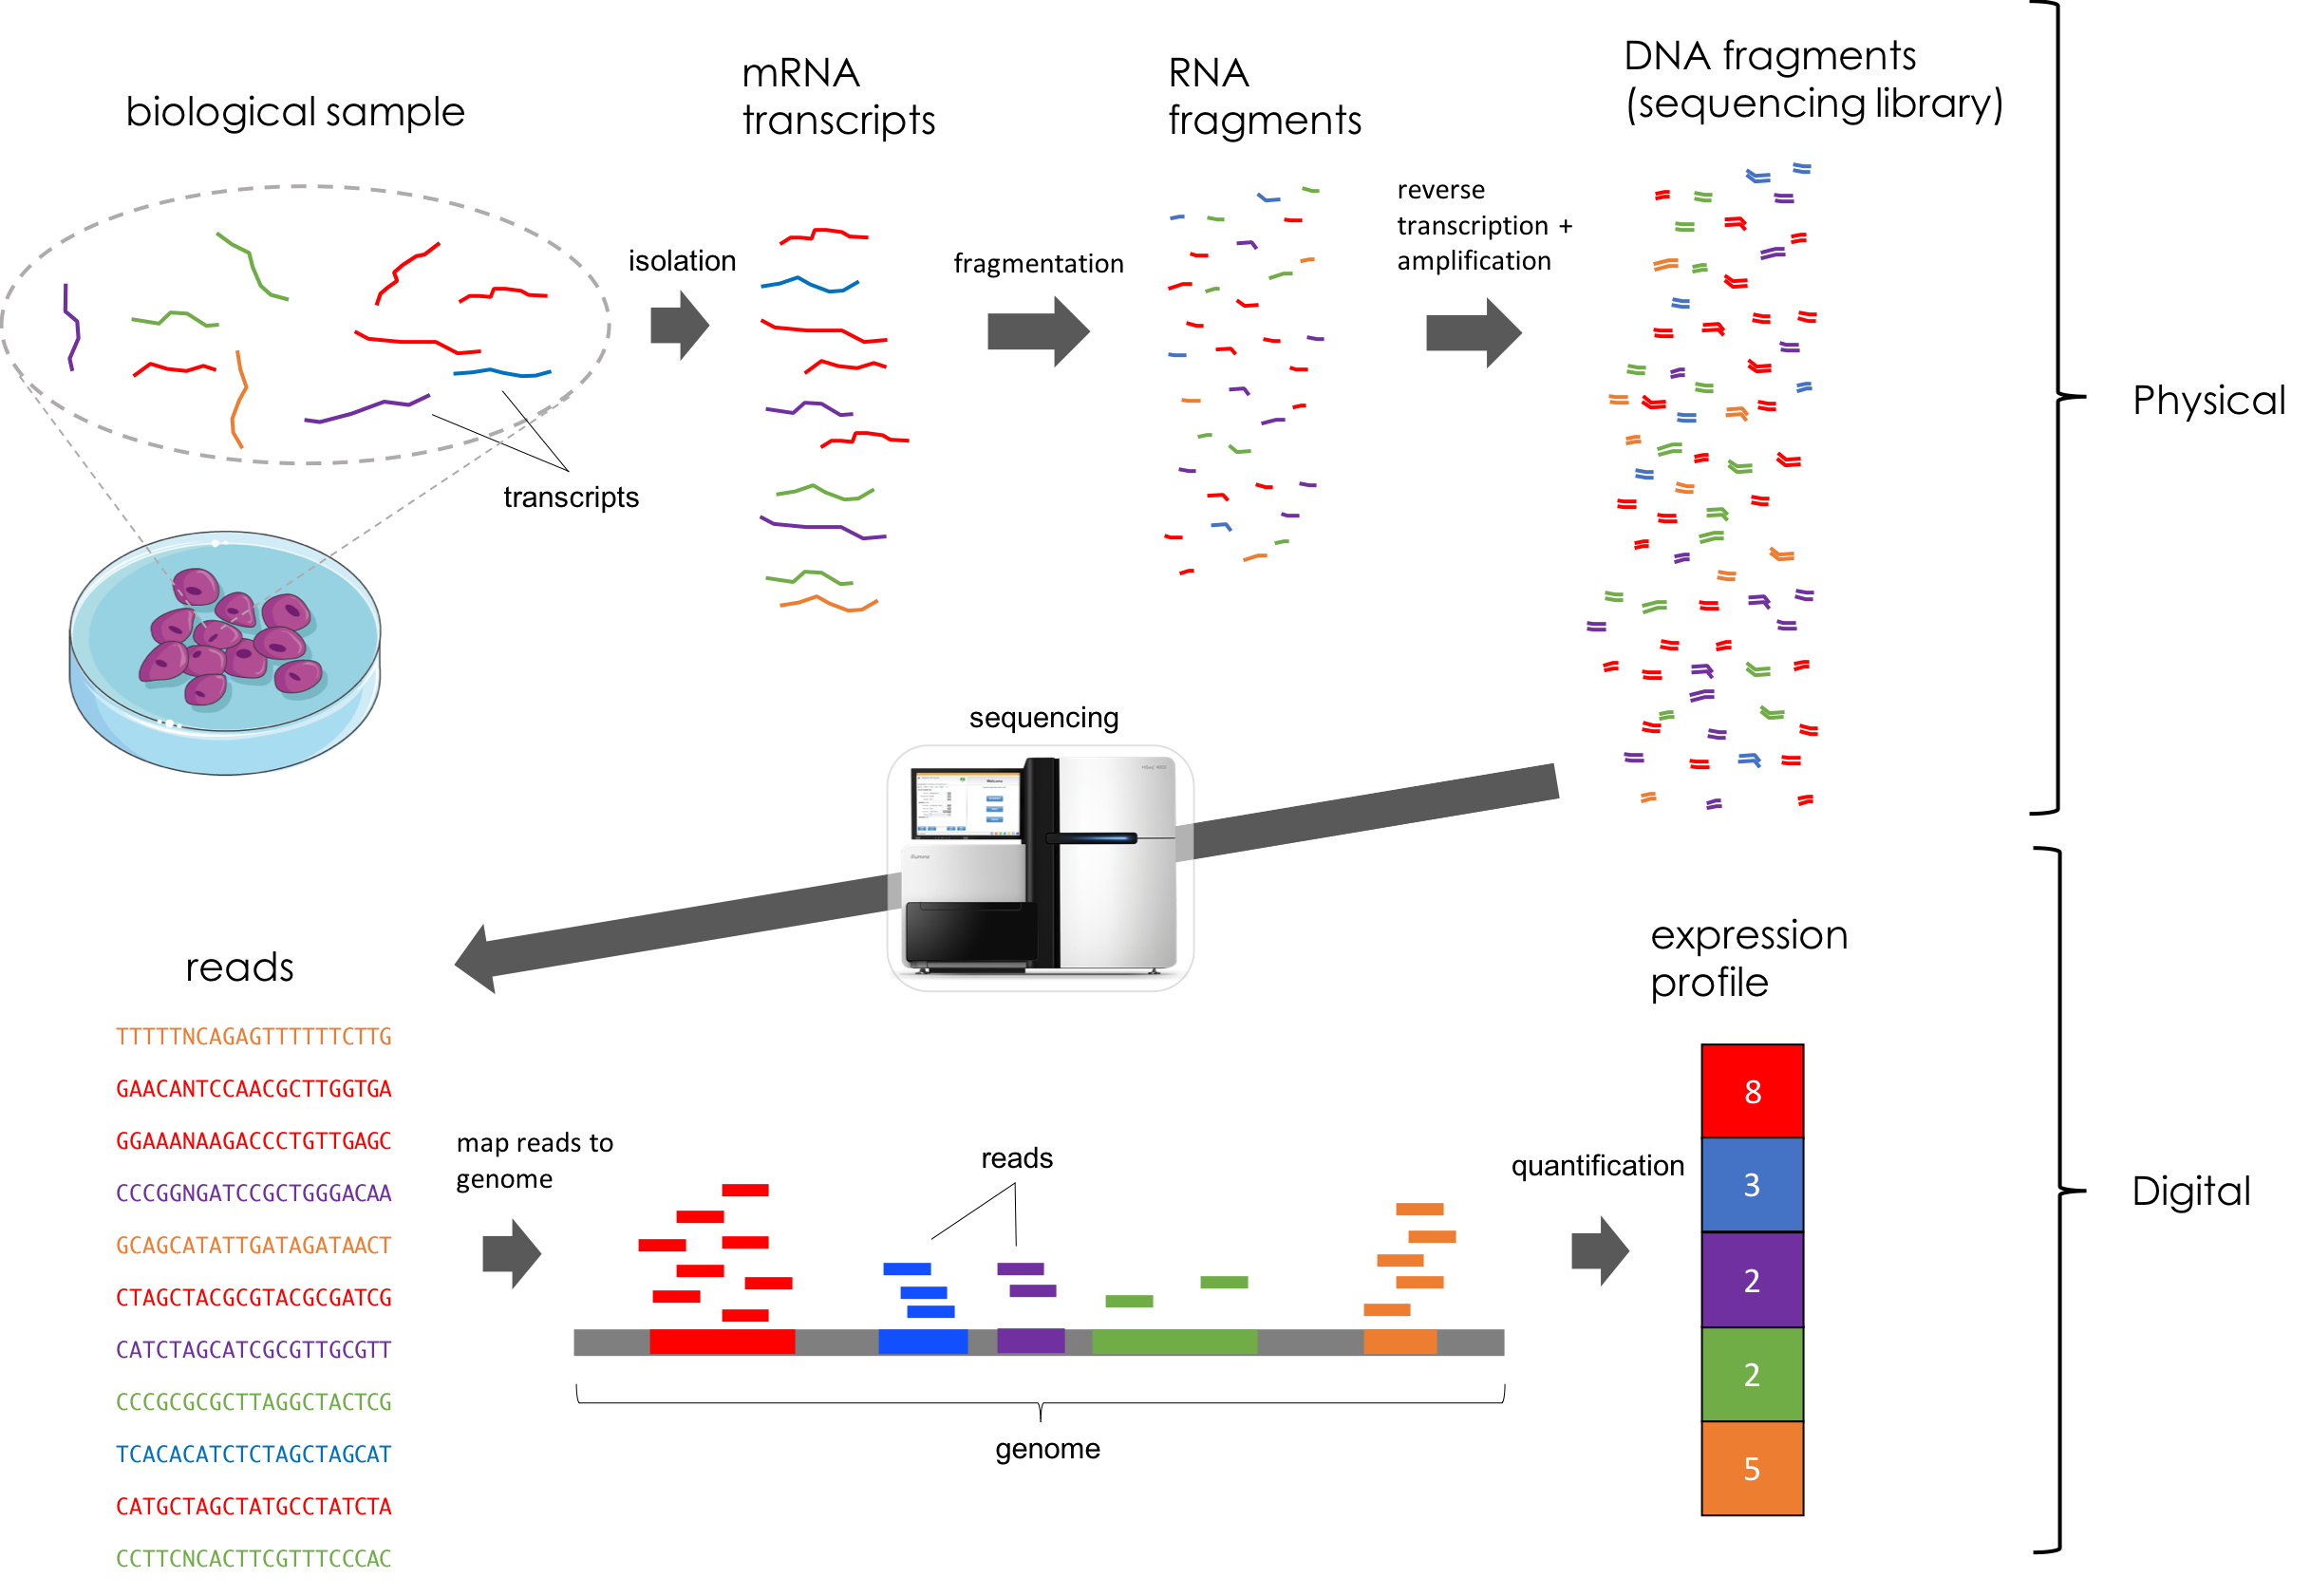
\includegraphics[scale=0.35]{figures/RNA_seq_schematic.png}}
\caption{\textbf{RNA-seq Overview.} A schematic illustrating a basic RNA-seq protocol. In this toy example there are five genes colored red, blue, green, orange, and purple. Each transcript and read is colored according to its gene of origin.}
\label{fig:rna_seq_protocol}
\end{figure*}


\section{Applications of transcriptome-based cellular phenotyping}

TBCP has a number of important applications.  In this section, we discuss some of these applications and notable efforts towards addressing them.

\subsection{Single-cell RNA-seq analysis}

In a traditional RNA-seq experiment, the RNA is isolated and pooled from a population of cells. In these \textit{bulk RNA-seq} experiments, only the average gene expression for the population can be obtained rather than the gene expression of individual cells.   Within the last several years, advances in microfluidics have enabled the development of new protocols, called \textit{single-cell RNA-seq} (scRNA-seq), that entail isolating and extracting RNA from individual cells, thereby allowing for the study of gene expression at the single-cell level (\citealp{Tang2009}).  scRNA-seq enables the study of cell populations at a level of granularity never before accessible, and is therefore leading to discoveries of new cell populations (\citealp{Aizarani2019, Plasschaert2018}) and new mechanisms that account for both healthy tissue function (\citealp{Tikhonova2019, Economo2018}) and disease (\citealp{Mathys2019, Vladoiu2019}).  Furthermore, these technologies are undergoing rapid development and are enabling the sequencing of ever-more cells per experiment. For example, one recent study generated expression profiles for over a hundred thousand cells (\citealp{TabulaMuris2018}).

Scientists who perform scRNA-seq commonly need to identify the cell type of each cell in their dataset.  We consider the task of developing automated systems for classifying cell types in scRNA-seq data to be a TBCP task where cell type is the phenotype of interest.  Traditionally, labeling cell types in scRNA-seq data is an ad hoc process that involves clustering the cells and then searching for differential expression of certain cell-type-specific marker genes across these clusters. This process is challenged both by the fact that there is not a canonical set of marker genes for most cell types (\citealp{Zhang2018}) and that this process is affected by the clustering algorithm (\citealp{Kiselev2019}). To address these issues, approaches are beginning to emerge that rely on training cell type classifiers  (\citealp{Hou2019, Kanter2019, Xie2019, Aran2019, Lieberman2018, Alavi2018, Lin2017}).  

\subsection{Stem cell engineering}

\textit{Stem cells} are a category of cells in multicellular organisms that are capable of converting themselves into more specialized cell types through a process called \textit{differentiation}.  Because of their plasticity, there is great interest in understanding and controlling this differentiation in order to direct cells into becoming a specific targeted tissue type (\citealp{Tewary2018}).  The ability to engineer cells from stem cells is heralding new therapies for regenerating and repairing diseased and injured tissue (\citealp{DeLuca2019}).  

When scientists develop these in vitro differentiation protocols, they must assess how well the differentiated cells resemble the targeted cell type in vivo. To assess this, scientists will often compare a number of characteristics, including gene expression, of their in vitro differentiated cells to fresh, primary cells. To this end, machine learning based TBCP methods have been developed to facilitate this comparison (\citealp{Roost2015, Cahan}).  The idea here is that a machine learning model can classify the cell type or tissue type of the in vitro differentiated cells and the classifier's prediction can inform the user as to what cell type or tissue type the differentiated cells resemble.  The user can then use this knowledge in the diagnoses of their differentiation protocols (\citealp{Morris2014}).
 
\subsection{Disease diagnosis}

Because the transcriptome plays a major role in determining the cell's state, disease processes are often associated with aberrations in the transcriptome.  Therefore, TBCP promises to be a powerful tool for clinical diagnosis (\citealp{Bryon2016}).  For example, in metastasized cancer, a first step in treatment determination is identifying the cancer's tissue of origin. To this end, researchers are exploring machine learning-based TBCP for identifying the tissue of origin in metastasized cancers (\citealp{Sun2018, Li2017}). Along similar lines, researchers are identifying new cancer subtypes, even within the same tissue (\citealp{Hoadley2018}). As the landscape of cancer subtypes is further revealed, new TBCP tools will be required to classify the subtype of tumors in order to better inform treatments (\citealp{Saddiki2015}).   

\subsection{Data curation}

As previously mentioned (and to be described in detail in Section~\ref{sec:intro_sra}), the NIH and other institutions maintain public databases, such as the SRA, for scientists to deposit their gene expression data to enable secondary analyses.  Oftentimes, data submitters will not adequately describe the phenotypes associated with their data leading to difficulty in performing these secondary analyses (\citealp{Goncalves2019, Goncalves2017}).  TBCP offers a path towards correcting or completing the phenotype-specific descriptions of these data. To this end, machine-learning based TBCP methods have been developed specifically for the purposes of curating public gene expression data (\citealp{Ellis, Lee2013})

\section{The Sequence Read Archive}\label{sec:intro_sra}

Because sample retrieval, preparation, and sequencing are expensive, the NIH created the SRA for scientists to deposit the raw reads from their experiments for the purposes of future secondary analyses. The SRA stores reads from a variety of sequencing assays, including RNA-seq.  It is important to note that the SRA is organized in a hierarchical fashion (Fig.~\ref{fig:sra_structure}). At the highest level, data is grouped by \textit{study} where a study represents a single scientific investigation.  Each study is then associated with a set of biological \textit{samples} (e.g., a biological replicate) in a one-to-many relationship. Each biological sample is then associated with a set of sequencing \textit{experiments} in a one-to-many relationship.  As of Summer 2019, the SRA stores over \NumSRAExperiments{} total human RNA-seq samples from over \NumSRASamples{} biological samples. These data belong to over \NumSRAStudies{} studies. 

There are a number of significant challenges that, to date, have significantly impeded our ability to use the SRA, and other related public databases, as a source of training data. First, the SRA does not dictate a set of standards for data submitters regarding the metadata that describes the sample-specific phenotypes.  This has led to the metadata containing many synonyms, misspellings, and references to outside information (\citealp{Goncalves2017}).  Because of this, researchers who wish to use public sources of gene expression data for training machine learning classifiers have been required to put forth a significant curation effort to generate standardized phenotype labels (\citealp{Alavi2018, Lee2013, Schmid2012}).

Second, obtaining gene expression profiles from the SRA's raw reads is challenging. As previously described, quantifying gene expression from the reads generated by RNA-seq requires mapping the reads to the genome.  Because a single RNA-seq experiment generates tens of millions of reads, this process is computationally expensive in terms of both time and memory.  Fortunately, recent advances in gene expression quantification algorithms are alleviating this computational burden (\citealp{Nellore2017, Patro2017, Bray2016}). This has lead to a number of efforts towards mass quantifying SRA RNA-seq data (\citealp{Lachmann2018, ColladoTorres2017}).

Third and finally, because the SRA consists of data from diverse scientific studies, analyses of these data must contend with \textit{batch effects} (\citealp{Leek2010}). Batch effects are technical effects or systemic errors that cause bias between groups of samples grown or sequenced under similar experimental conditions.  Batch effects can account for a significant amount of variation in RNA-seq data, especially in public data where ``batches" are considered to be groups of samples that share a scientific study of origin. Specifically, one often finds that data in the diverse datasets such as the SRA predominantly cluster according to their study rather than according to their phenotype (Fig.~\ref{fig:batch_effects}).  When constructing and analyzing methods for TBCP using public data, these batch effects must be taken into account.  For example, in order to assess the true generalization performance of a trained classifier, it is important to test the classifier on data from studies that differ from the studies used in the training set  (\citealp{Bernau2014}). Failing to do so will lead to an overly optimistic measurement of performance of the algorithm due to the fact that the test set unrealistically resembles the training set. 

\begin{figure*}[!tpb]
\centerline{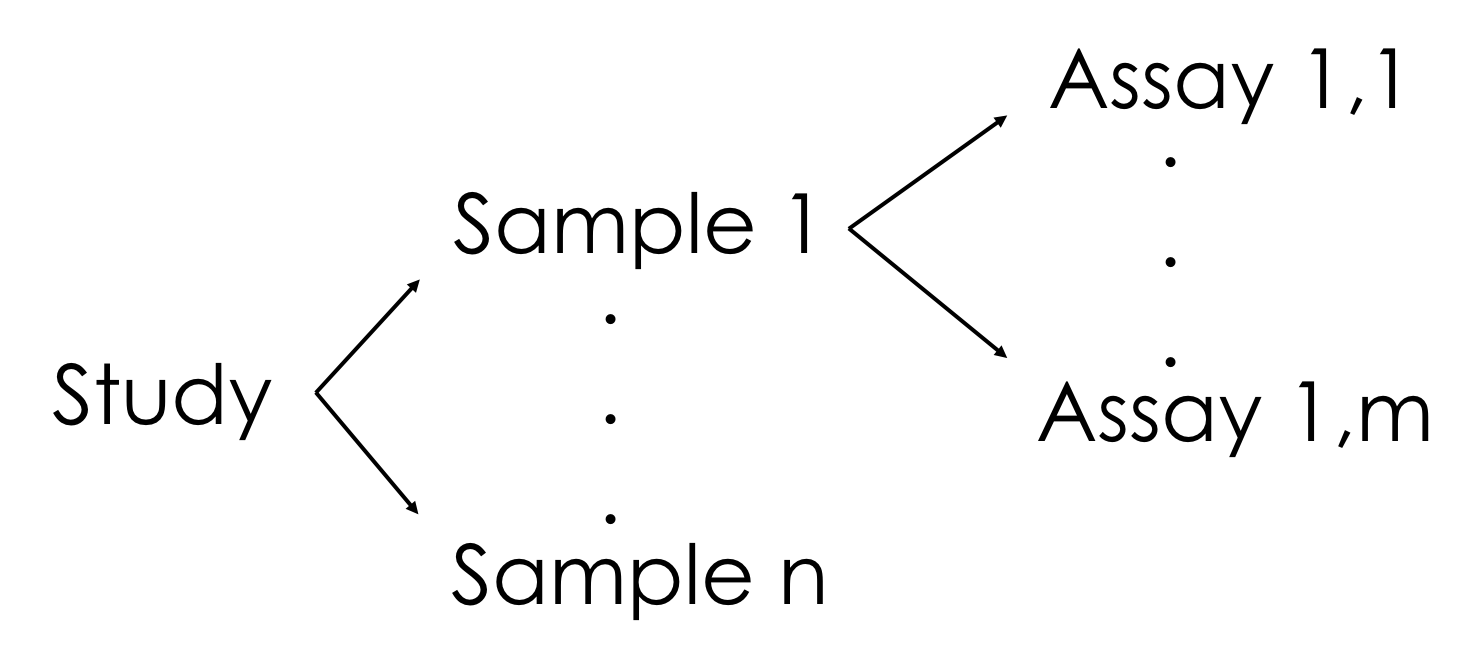
\includegraphics[scale=0.4]{figures/SRAStructure.png}}
\caption{\textbf{Structure of the SRA.} A schematic illustrating the hierarchical structure of the Sequence Read Archive.}
\label{fig:sra_structure}
\end{figure*}

\begin{figure*}[!tpb]
\centerline{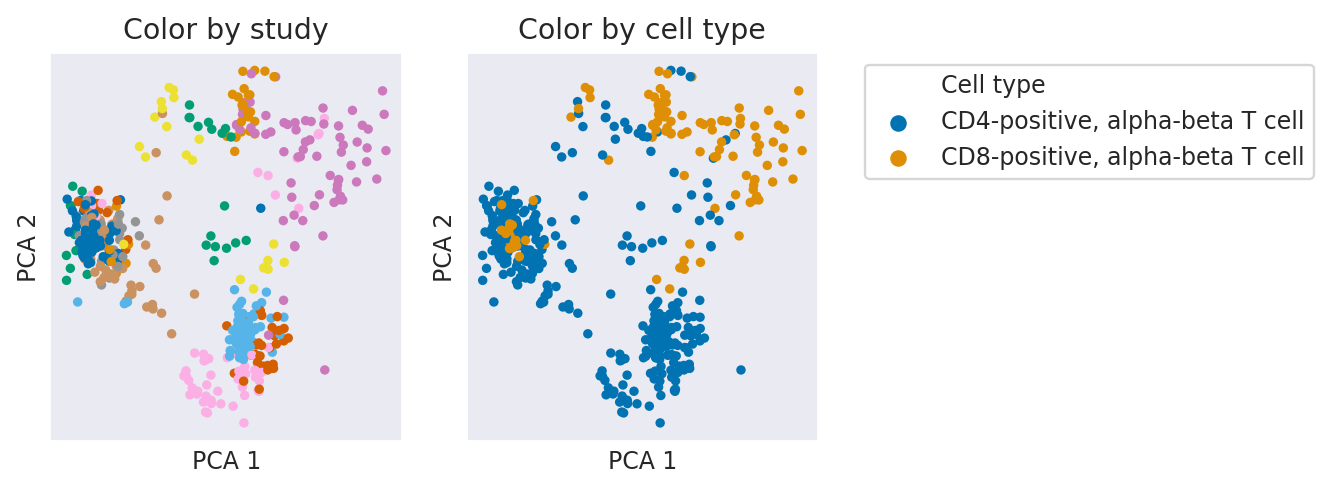
\includegraphics[width=13cm]{figures/batch_effects.png}}
\caption{\textbf{PCA plots illustrating batch effects.} PCA plots of curated CD4-positive T cell and CD8-positive T cell bulk RNA-seq samples from the SRA (described in Section~\ref{sec:primary_cell_data}). In the left-hand figure each point is colored according to the sample's study. The legend on the right pertains only to the right-hand figure.  On the right-hand figure, these same points are colored according to their cell type. Ideally, one find two tight clusters pertaining to the two presented cell types. Rather, as seen above, the clusters are largely explained by their study thus providing an example of batch effects.}
\label{fig:batch_effects}
\end{figure*}


\section{Encoding phenotypes using ontologies}

The projects presented in this work make extensive use of biomedical ontologies.  An \textit{ontology} is a structured knowledge-base that defines a set of concepts/terms within a specific domain of discourse. Besides providing the definition for each term, an ontology also encodes a directed acyclic graph (DAG) (Fig.~\ref{fig:onto_schem}) in which each term is represented by a node and each edge represents a relationship between two terms. Edges are usually labelled with a relationship-type. For example, the most common edge is the "\texttt{is\_a}" edge. Given terms $a$ and $b$, $a$ \texttt{is\_a} $b$ asserts that all instances of $a$ are also instances of $b$. Similarly, the "\texttt{part\_of}" edge represents the knowledge that one entity is a component of another entity.   

\begin{figure*}[!tpb]
\centerline{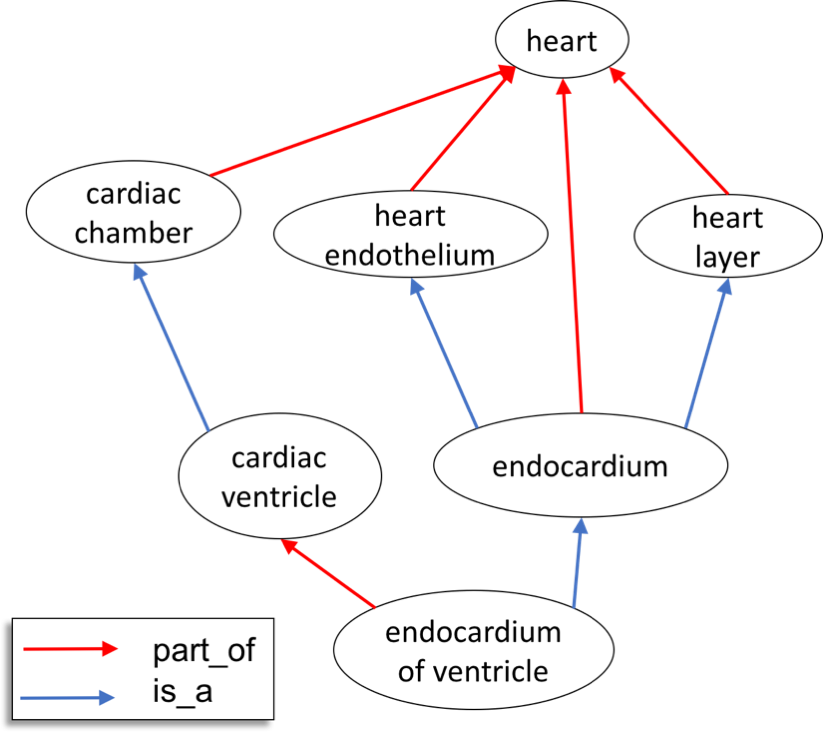
\includegraphics[scale=0.68]{figures/onto_schematic.png}}
\caption{\textbf{Example ontology graph.} A subgraph from the Uberon ontology representing anatomical entities in the heart. Red edges represent a \texttt{part\_of} relationship between terms. Blue edges represent an \texttt{is\_a} relationship between terms. }
\label{fig:onto_schem}
\end{figure*}

The fact that ontologies are hierarchically structured provides a number of advantage for the description and retrieval of public data. First, since the public data is highly diverse, the hierarchical structure enables a standardized description of data across the multiple levels of specificity of phenotypes in the database.  For example, a biological sample consisting of T cells can be labelled as ``T cell" while another sample consisting of the more specific cell type CD4-positive T cells can be labelled using a more specific term. Furthermore, the hierarchical structure also facilitates querying these diverse data. In the example above, a query for all T cells will return both samples labelled as ``T cell" and those labelled as ``CD4-positive T cell" due to ``CD4-positive T cell" being a descendant of the query in the ontology's DAG.



\section{Hierarchical multi-label classification}

Because our phenotypes are encoded as a hierarchy, the projects presented in this dissertation frame the machine learning-based TBCP task as that of \textit{hierarchical multi-label classification}.  (Fig.~\ref{fig:hierarchical_classification}).  More formally, multi-label classification is the task of learning a function 
$$f: \mathcal{X} \rightarrow \mathcal{P}(\mathcal{Y})$$ 
where $\mathcal{X}$ is the set of all possible items (in our case, $\mathcal{X} := \mathbb{R}^G$ is the set of all possible RNA-seq derived expression profiles) , $\mathcal{Y}$ is the set of all possible labels (in our case, phenotypes), and $\mathcal{P}(\mathcal{Y})$ is the powerset of $\mathcal{Y}$.  That is, given an item $x \in \mathcal{X}$, we assign $x$ a subset of labels $f(x) \subseteq\mathcal{Y}$.  Provided a DAG over the labels $Y$, hierarchical, multi-label classification imposes the restriction on $f$ that given an item $x$ and label $y \in f(x)$, the parents of $y$ in the DAG are also in $f(x)$.

Framing the TBCP task as hierarchical classification presents a number of advantages over "flat" classification in which the ontology terms are not structured hierarchically. First, the DAG of an ontology provides a rich source of prior knowledge to the classification task that remains un-utilized in flat classification.  By utilizing the hierarchy during training rather than using flat classification, more accurate classifiers can be learned (\citealp{BarutcuogluSchapireTroyanskaya2006}). Second, hierarchical classification allows for informative predictions to be made on query samples whose true phenotype label may not be included in the ontology either because the ontology is incomplete or that phenotype has yet to be discovered. Take for example the small hierarchy in Figure~\ref{fig:hierarchical_classification} encoding T cell types in the Cell Ontology (\citealp{Bard})\footnote{T cells play a pivotal role in the immune system.  They are responsible for detecting and responding to infection as well as for priming the immune system to respond to future attacks.}.  In the hypothetical scenario in which the "$\gamma\delta$ T cell"  is not in the ontology, a hierarchical classifier could label a sample of this cell type as "T cell", which would be the most apt cell type term of those available. Lastly, the use of hierarchical classification approaches allows for the placement of a bulk RNA-seq sample at a level of the hierarchy appropriate to its heterogeneity. For example, a population of cells enriched for T cells may be heterogeneous in the sub-types of T cells (e.g., $\alpha\beta$ CD4+ T cells and $\alpha\beta$ CD8+ T cells). In this case, "T cell" would be the most apt prediction.

\begin{figure*}[!tpb]
\centerline{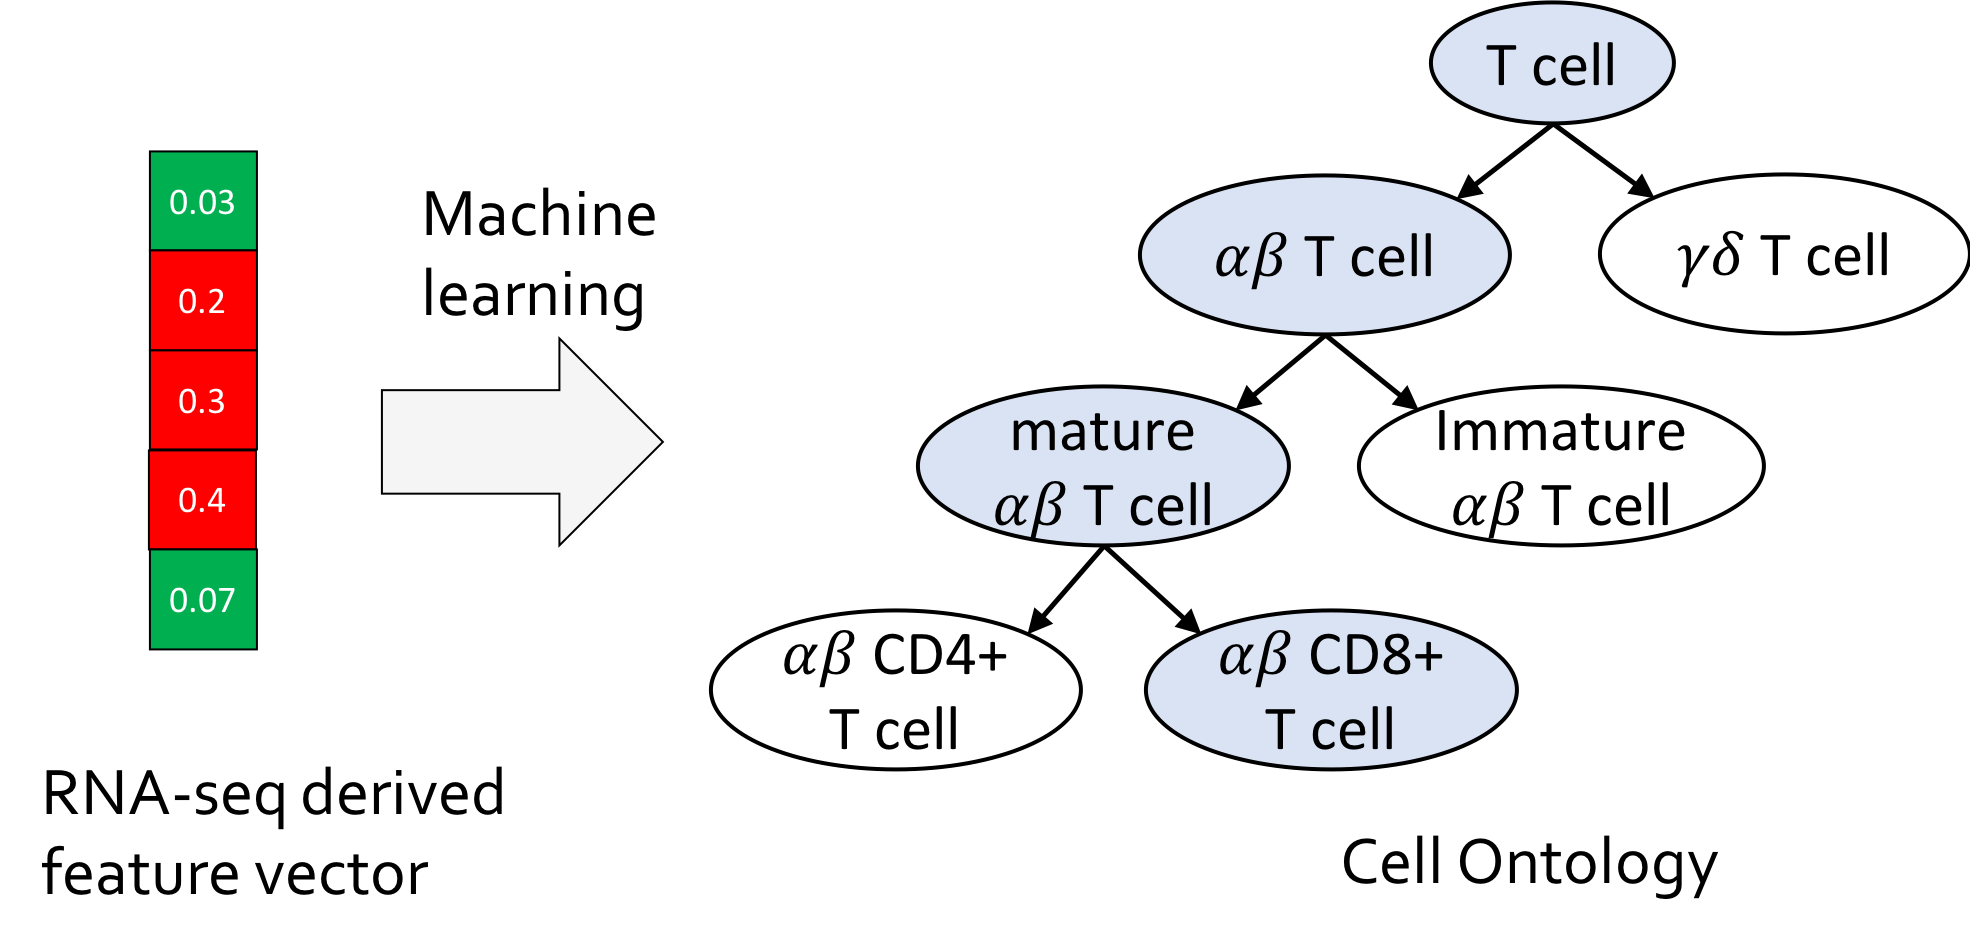
\includegraphics[width=13cm]{figures/hierarchical_classification.png}}
\caption{\textbf{Hierarchical classification.} A schematic illustrating hierarchical classification. Given an input vector of gene expression values (red indicates the gene is highly expressed and green indicates the gene is lowly expressed), the algorithm outputs a set of predicted ontology terms following the structure of the ontology (the shaded nodes on the right).}
\label{fig:hierarchical_classification}
\end{figure*}

Hierarchical classification algorithms can roughly be divided into two categories: \textit{ensemble-based} approaches and \textit{global} approaches (\citealp{Silla2011}).  Ensemble-based approaches entail training a set of independent "flat" classifiers, where each classifier corresponds to a node of the hierarchy, and then aggregating the outputs of these classifiers so that they are consistent with the hierarchy\footnote{Because each classifier makes a prediction independently from the rest, these predictions may be logically inconsistent with the hierarchy. This will occur if a classifier outputs a positive prediction for a given node, but it's parent classifier outputs a negative prediction.}.  Ensemble-based approaches can be further divided according to how each flat classifier is trained. Some methods train independent one-vs.-rest classifiers for each node, where each classifier makes a binary decision as to whether the query instance belongs to the given node or not. Examples of these approaches include Baysian Network Correction (\citealp{BarutcuogluSchapireTroyanskaya2006}) and projection-based approaches (\citealp{Obozinski2008}).  Other ensemble-based approaches take a different strategy in which classification is performed in a top-down fashion and each node's classifier makes a binary decision as to whether the query item belongs to the given node conditioned on the fact that it belongs to the parents of that node (\citealp{Obozinski2008, CesaBianchi2006}). In contrast, in the global approach, classification is inextricably intertwined with the hierarchy of the labels. Examples of global approaches include decision tree-based approaches (\citealp{Vens2008}), supervised hierarchical latent Dirichlet allocation (\citealp{Perotte2011}), and kernel dependency estimation approaches (\citealp{Bi2011}).  
  
In this work, we explore ensemble-based approaches because they admit more flexibility in their development. This is because, in contrast with global approaches, ensemble-based approaches decouple the hierarchical classification process into two steps: first, each independent classifier makes its predictions and then these predictions are aggregated to ensure that they are consistent with the hierarchy.  Thus, the design decisions regarding the independent classifiers are independent from the design decisions regarding how the predictions are made to be consistent with the hierarchy. 

\section{This dissertation}

In this section, we outline the contributions presented in this thesis.  These contributions span multiple stages of the machine learning pipeline, from acquiring labelled training data (Chapter~\ref{chap:1}), to developing machine learning algorithms (Chapters \ref{chap:2} and \ref{chap:3}) (Fig.~\ref{fig:phenotyping_dataflow}).  We preview the contributions of this thesis in the subsections below:
 
\subsection{Normalized sample-specific metadata for the SRA}

In the first project, we address the challenge of obtaining ground-truth, labeled training data from the SRA for performing supervised training of a phenotype classifier. Such ground truth labelings are difficult to obtain due to the poor structure of the sample-specific metadata in the SRA.  In this project we developed a novel computational approach for normalizing this metadata by tagging sample entries in the SRA with terms from biomedical ontologies. Existing approaches treat metadata normalization as a \textit{named entity recognition} (NER) problem, where the goal is to tag metadata with terms from controlled vocabularies when that term is mentioned explicitly in the metadata text. We reframed this problem as an inference task, in which we seek to tag the metadata with only those terms that describe the underlying biology of the described sample rather than tag the metadata with all mentioned terms. We found that this approach yielded mapped ontology terms with fewer false positives than existing approaches that frame the problem as NER. 

\subsection{Hierarchical cell type classification using mass, heterogeneous RNA-seq data from human primary cells}

In the second project, we use the mapped ontology terms produced by the first project in order to supervise the training of RNA-seq-based phenotype classifiers. We specifically focus on the cell type prediction task: given an RNA-seq sample, we wish to predict the cell type from which the sample was derived.  Cell type prediction is an important step in many transcriptomic analyses, including that of annotating cell types in single-cell RNA-seq datasets. This work represents the first concerted effort towards the cell type  prediction task that utilizes the full potential of publicly available RNA-seq data.  Further, we explore the novel application of hierarchical machine learning classifiers to leverage prior knowledge of cell type hierarchies, specifically, the Cell Ontology. To this end, we pushed the state-of-the-art in cell type prediction accuracy of bulk and single-cell RNA-seq.  

\subsection{Cell type classification of sparse single-cell RNA-seq data}

In the third project, we build on the second project in order to address the task of cell type prediction on \textit{sparse} scRNA-seq data from novel droplet-based technologies.  These droplet-based scRNA-seq technologies are enabling the sequencing of higher numbers of cells at the cost of a lower read-depth per cell, which results in expression measurements for fewer genes per cell.  In this project, we explore the effects of applying cell type classifiers trained on dense, bulk RNA-seq data to sparse scRNA-seq data and propose a novel probabilistic generative model for adapting the bulk-trained classifiers to sparse input.

\begin{figure*}[!tpb]
\centerline{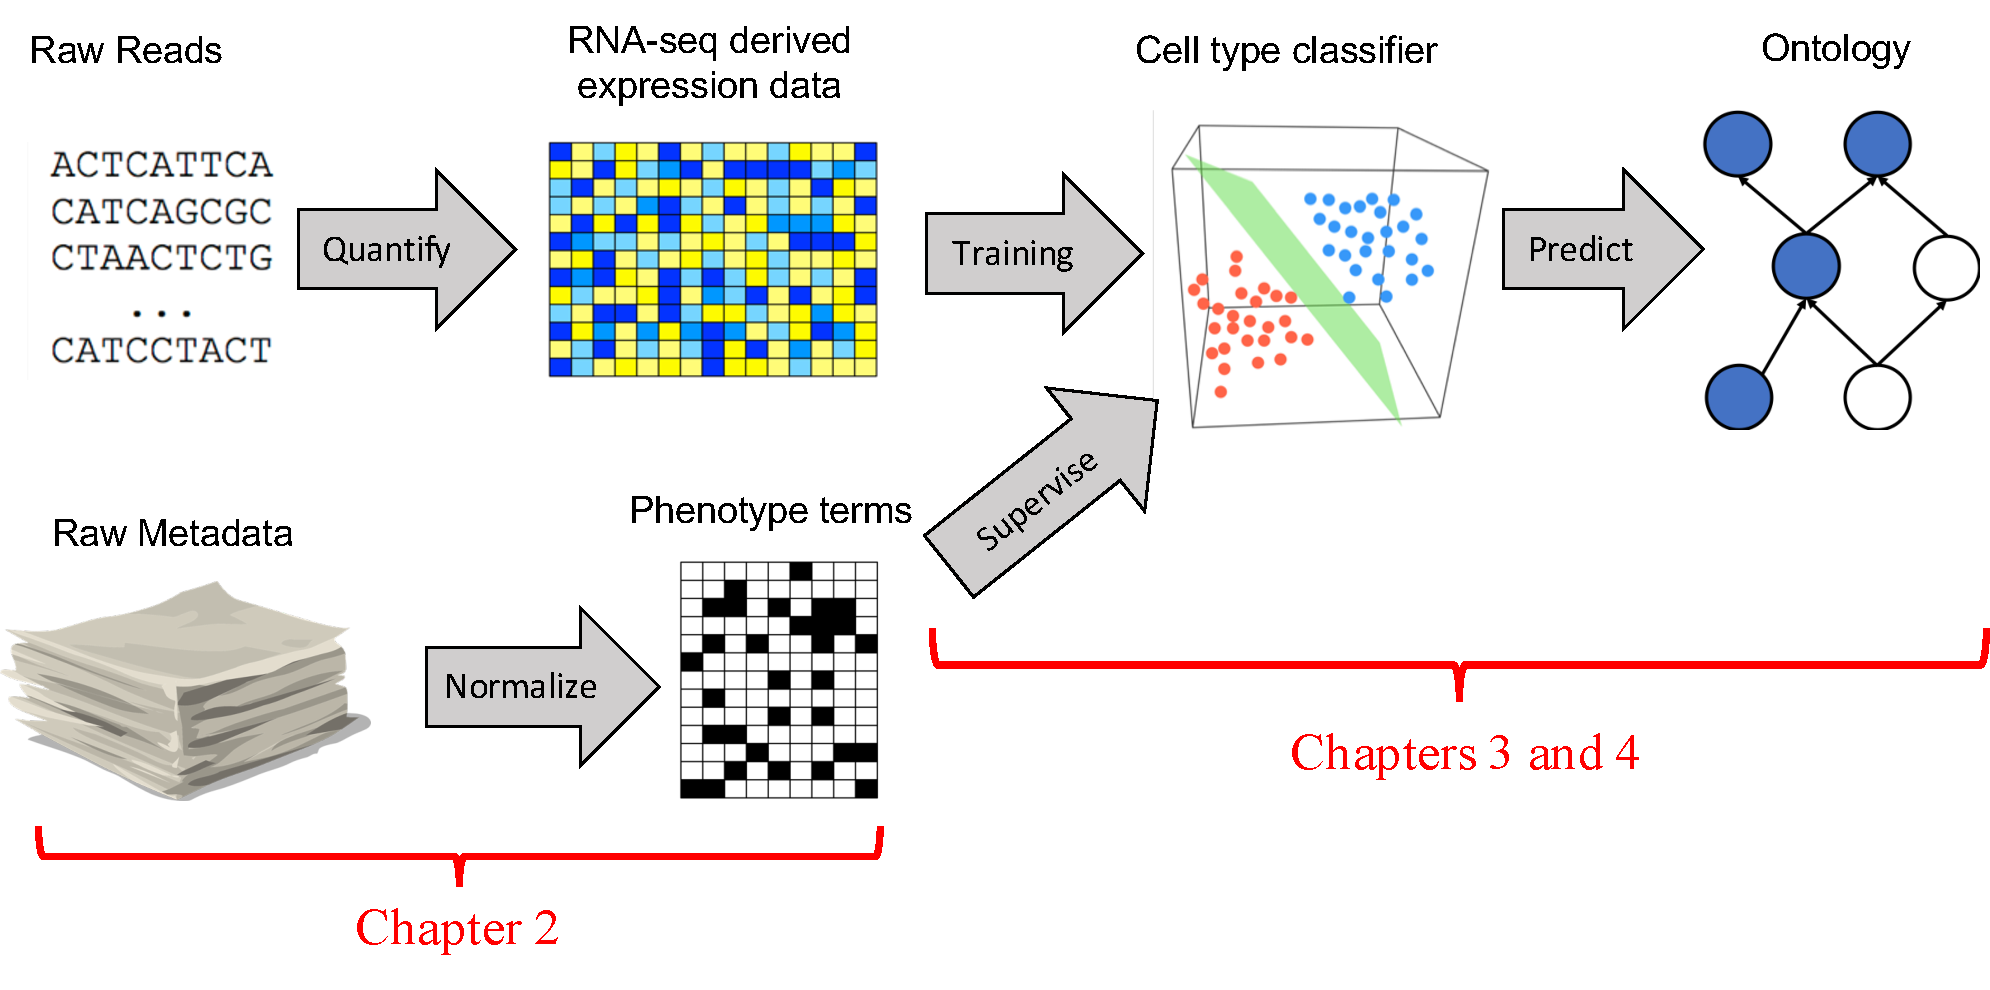
\includegraphics[width=13cm]{figures/phenotyping_dataflow.pdf}}
\caption{\textbf{TBCP Overview.} A schematic illustrating the components of the transcriptome-based cellular phenotyping task.}
\label{fig:phenotyping_dataflow}
\end{figure*}




%However, these opportunities are impeded by a number of challenges including poorly structured metadata and data heterogeneity.  In this thesis, I present three related projects that address these challenges via the development of novel computational methodologies. 


















